\chapter{Xây dựng chương trình \& Kết quả}

Chương này là sẽ trình quá trình xây dựng một chương trình ứng dụng hoàn chỉnh cho việc nhận dạng hóa đơn thông qua công nghệ OCR và kết quả đạt được của chương trình.
\section{Ý tưởng}
Để xây dựng được một chương trình hoàn chỉnh cho đề tài ``\textbf{Nghiên cứu ứng dụng OCR nhận dạng hóa đơn}'', chương trình sẽ cần sự kết hợp của nhiều mô hình với các nhiệm vụ khác nhau để tạo thành một chương trình hoàn chỉnh Hình \ref{pipeline}. Ý tưởng của chương trình này là từ bức ảnh đầu vào ảnh sẽ cho qua các bước tiền xử lý hình ảnh để tăng chất lượng ảnh đầu vào tiếp đến ảnh sẽ được cho qua bước phát hiện văn bản ở bước này đầu ra của ảnh sẽ là các 4 điểm tọa độ $(x, y)$ của vùng văn bản đã được mô hình phát hiện, các điểm này sẽ được dùng làm đầu vào cho mô hình nhận dạng văn bản và KIE. Bước nhận dạng sẽ dự đoán văn bản trong vùng được phát hiện còn KIE sẽ thực hiện phân loại nhãn cho vùng văn văn bản. Sau đó cả hai sẽ được qua hàm hậu xử lý để cải thiện chất lượng và độ chính xác của văn bản dễ dàng cho các bước tiếp. Trích xuất các thông tin quan trọng và trực quan hóa hình ảnh, đưa về dữ liệu có cấu trúc \ldots
\begin{figure}
    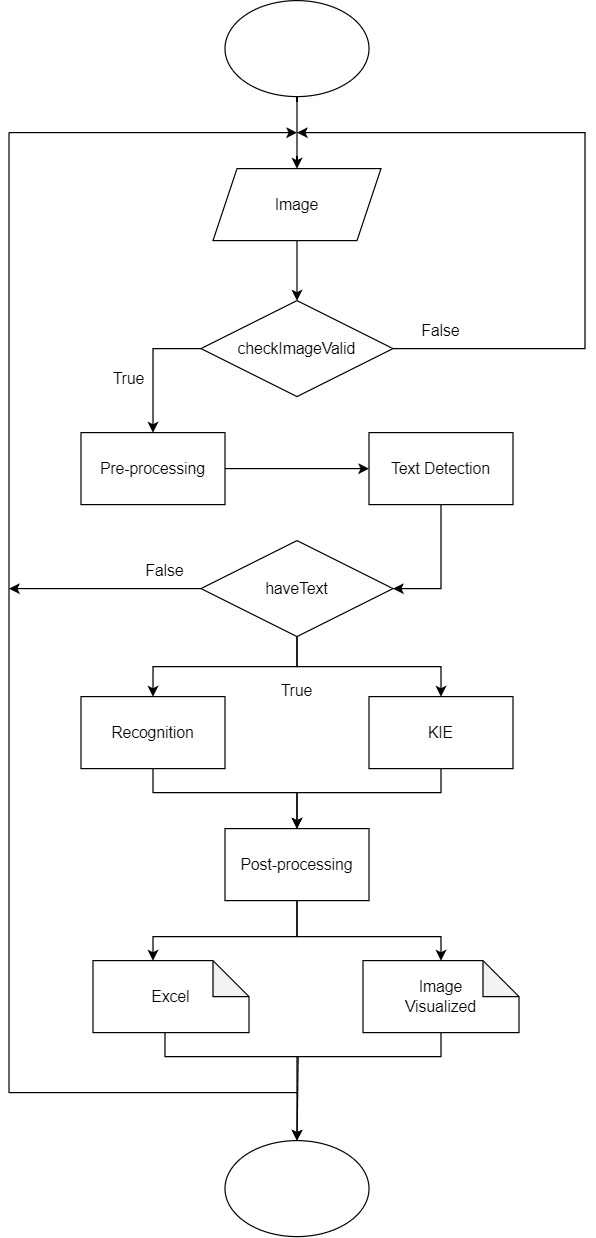
\includegraphics[scale=0.53]{images/pipeline.png}
    \centering
    \caption{Lưu đồ của chương trình nhận dạng hóa đơn}
    \label{pipeline}
\end{figure}

\newpage
\section{Xây dựng chương trình}
\subsection{Tiền xử lý ảnh}

\begin{lstlisting}[language=Python]
def preprocess_image(_image):
    _image = alpha_to_color(_image, alpha_color)
    # Gaussian blur
    _image = cv2.GaussianBlur(_image, (1,1), cv2.BORDER_DEFAULT)

    # Image Sharpness
    kernel = np.array([[-1,-1,-1], 
                       [-1, 9,-1], 
                       [-1,-1,-1]])
    _image = cv2.filter2D(_image, -1, kernel)
    if inv:
        _image = cv2.bitwise_not(_image)
    if bin:
        _image = binarize_img(_image)
    return _image  
\end{lstlisting}

Ở đoạn code trên em sử dụng các phương pháp tiền xử lý ảnh cơ bản, để cải thiện chất lượng ảnh đầu vào cho chương trình.
\subsection{Phát hiện vùng văn bản} \label{detsec}
Đoạn code dưới đây sử dụng thư viện PaddleOCR để xây dựng một ứng dụng phát hiện văn bản trong hình ảnh.
\begin{lstlisting}[language=Python]
from paddleocr import PaddleOCR

self.ocr_engine = PaddleOCR(
    use_angle_cls=False,
    show_log=False,
    det_model_dir=global_config.get("kie_det_model_dir", None),
    use_gpu=global_config['use_gpu'])

det_result = self.ocr_engine(image)
\end{lstlisting}
Kết quả trả về là một danh sách các điểm tọa độ
\begin{lstlisting}[language=Python]
[[27.0, 459.0], [136.0, 459.0], [136.0, 479.0], [27.0, 479.0]]
[[28.0, 429.0], [372.0, 429.0], [372.0, 445.0], [28.0, 445.0]]
......
\end{lstlisting}

\subsection{Nhận dạng văn bản}
Với nhận dạng hóa đơn đầu vào của nhiệm vụ này là kết quả của \ref{detsec}. Hàm \texttt{recog} nhận 2 tham số đầu vào là ảnh đầu vào, và các điểm tọa độ, hàm sẽ thực hiện lấy các vùng văn bản và thực hiện dự đoán các văn bản trong từng \texttt{roi}.
\begin{lstlisting}[language=Python]
from src.ocr.tools.predictor import Predictor
from src.ocr.tools.config import Cfg

self.config = Cfg.load_config_from_file(global_config['rec_config_path'])
self.config['predictor']['import'] = global_config['rec_weight']
self.config['predictor']['beamsearch'] = True
self.config['cnn']['pretrained'] = False
self.config['device'] = 'cuda' if global_config['use_gpu'] else 'cpu'
self.detector = Predictor(self.config)

def recog(image, boxes):
    texts = []
    for box in tqdm(boxes):
        x, y, w, h = box
        roi = Image.fromarray(image[y:h, x:w])
        text = self.detector.predict(roi)
        texts.append(text)
    return text

self.recog(image, det_result)

\end{lstlisting}

Kết quả trả về của nhiệm vụ này là list các văn bản đã được dự đoán như hình dưới đây.
\begin{lstlisting}[language=Python]
['Okono', 'Số 85 Lê Văn Hiến, Đức Thắng, Bắc Từ Liêm', 'PHIÊU BÁN HÀNG/ INVOICE', 'Số:A3 1AA145550Ngày:18/05/2023 7:51:19PM', ...]
\end{lstlisting}
\subsection{KIE}
Đoạn mã sau thực hiện quy trình dự đoán phân loại thông tin trong hình ảnh, từ việc chuẩn bị dữ liệu đến việc thực hiện dự đoán và xử lý kết quả sau khi dự đoán.
\begin{lstlisting}[language=Python]
from ppocr.data import create_operators, transform
from ppocr.modeling.architectures import build_model
from ppocr.postprocess import build_post_process

self.post_process_class = build_post_process(config['PostProcess'],
                                             global_config)
self.model = build_model(config['Architecture'])

transforms = []
for op in config['Eval']['dataset']['transforms']:
    op_name = list(op)[0]
    if 'Label' in op_name:
        op[op_name]['ocr_engine'] = self.ocr_engine
    elif op_name == 'KeepKeys':
        op[op_name]['keep_keys'] = [
            'input_ids', 'bbox', 'attention_mask', 'token_type_ids',
            'image', 'labels', 'segment_offset_id', 'ocr_info',
            'entities'
        ]
    transforms.append(op)

if config["Global"].get("infer_mode", None) is None:
    global_config['infer_mode'] = True
self.ops = create_operators(config['Eval']['dataset']['transforms'],
                            global_config)
self.model.eval()

batch = transform(data, self.ops)
batch = to_tensor(batch)
preds = self.model(batch)
post_result = self.post_process_class(
            preds, segment_offset_ids=batch[6], ocr_infos=batch[7])
\end{lstlisting}
Kết quả sẽ trả về một danh sách các dictionary như sau:
\begin{lstlisting}[language=Python]
[[{'transcription': 'Okono', 'bbox': [435, 195, 811, 338], 'points': [[437.0, 195.0], [811.0, 201.0], [808.0, 338.0], [435.0, 332.0]], 'pred_id': 1, 'pred': 'SELLER'}, {'transcription': 'Số 85 Lê Văn Hiến, Đức Thắng, Bắc Từ Liêm', 'bbox': [309, 390, 890, 426], 'points': [[309.0, 390.0], [890.0, 392.0], [890.0, 426.0], [309.0, 424.0]], 'pred_id': 3, 'pred': 'ADDRESS'},...]
\end{lstlisting}
\subsection{Post-process}
Đoạn mã sau có chức năng xử lý và trích xuất thông tin từ kết quả của quá trình nhận dạng hóa đơn, sau đó tạo một Pandas DataFrame để lưu trữ thông tin này và xuất ra một tệp Excel

\begin{lstlisting}[language=Python]
def process_info(self, results):
    info = {
        'SELLER': '',
        'ADDRESS': '',
        'STAFF': '',
        'TIMESTAMP': '',
        'CODE': '',
        'PRODUCTS': [],
        'TOTAL_COST': 0
    }
    
    current_product = {
        'PRODUCT': '',
        'NUMBER': 0,
        'PRICE': 0
    }
    
    products = []
    for result in results:
        label = result['pred']
        transcription = result['transcription']
        
        if label != 'O':
            if label in ['PRODUCT', 'NUMBER', 'PRICE']:
                if label == 'PRODUCT':
                    current_product['PRODUCT'] = transcription
                    products.append(current_product.copy())
                else:
                    products[-1][label] = transcription
            else: 
                if label == 'TIMESTAMP':
                    text = transcription
                    code, time = text.split('Ngày')
                    info['CODE'] = code.strip()
                    info['TIMESTAMP'] = time[1:]
                else:
                    info[label] = transcription
                    
    info['PRODUCTS'] = products 

    product_rows = []
    for product in info_["PRODUCTS"]:
        product_row = [info_["SELLER"], info_["ADDRESS"], info_["STAFF"], info_["TIMESTAMP"], info_["CODE"],
                    product["PRODUCT"], product["NUMBER"], product["PRICE"], info_["TOTAL_COST"]]
        product_rows.append(product_row)

    # Create a Pandas DataFrame
    columns = ["SELLER", "ADDRESS", "STAFF", "TIMESTAMP", "CODE", "PRODUCT", "NUMBER", "PRICE", "TOTAL_COST"]
    df = pd.DataFrame(product_rows, columns=columns)

    # Create an Excel file
    now = datetime.now()

    current_time = now.strftime("%H-%M-%S")
    output_file = "invoice-{}.xlsx".format(current_time)
    df.to_excel(output_file, index=False, engine="openpyxl")

    print(f"Excel file '{output_file}' created.")

    return json.dumps(info, indent=1, ensure_ascii=False)
\end{lstlisting}

Đoạn mã sau vẽ kết quả của chương trình lên trên hình ảnh gốc.
\begin{lstlisting}[language=Python]
def draw_ser_results(image, ocr_results, 
                     font_path="doc/fonts/BeVietnamPro-Black.ttf", font_size=14):
    np.random.seed(2021)
    color = (np.random.permutation(range(255)),
             np.random.permutation(range(255)),
             np.random.permutation(range(255)))
    color_map = {
        idx: (color[0][idx], color[1][idx], color[2][idx])
        for idx in range(1, 255)
    }
    if isinstance(image, np.ndarray):
        image = Image.fromarray(image)
    elif isinstance(image, str) and os.path.isfile(image):
        image = Image.open(image).convert('RGB')
    img_new = image.copy()
    draw = ImageDraw.Draw(img_new)

    font = ImageFont.truetype(font_path, font_size, encoding="utf-8")
    for ocr_info in ocr_results:
        if ocr_info["pred_id"] not in color_map:
            continue
        color = color_map[ocr_info["pred_id"]]
        text = "{}: {}".format(ocr_info["pred"], ocr_info["transcription"])

        if "bbox" in ocr_info:
            bbox = ocr_info["bbox"]
        else:
            bbox = trans_poly_to_bbox(ocr_info["points"])
        draw_box_txt(bbox, text, draw, font, font_size, color)

    img_new = Image.blend(image, img_new, 0.7)
    return np.array(img_new)    
\end{lstlisting}

\newpage
\section{Kết quả}
Dưới đây là một số kết quả đạt được của đề tài:
\paragraph*{Kết quả 1}
\begin{figure}[h]
    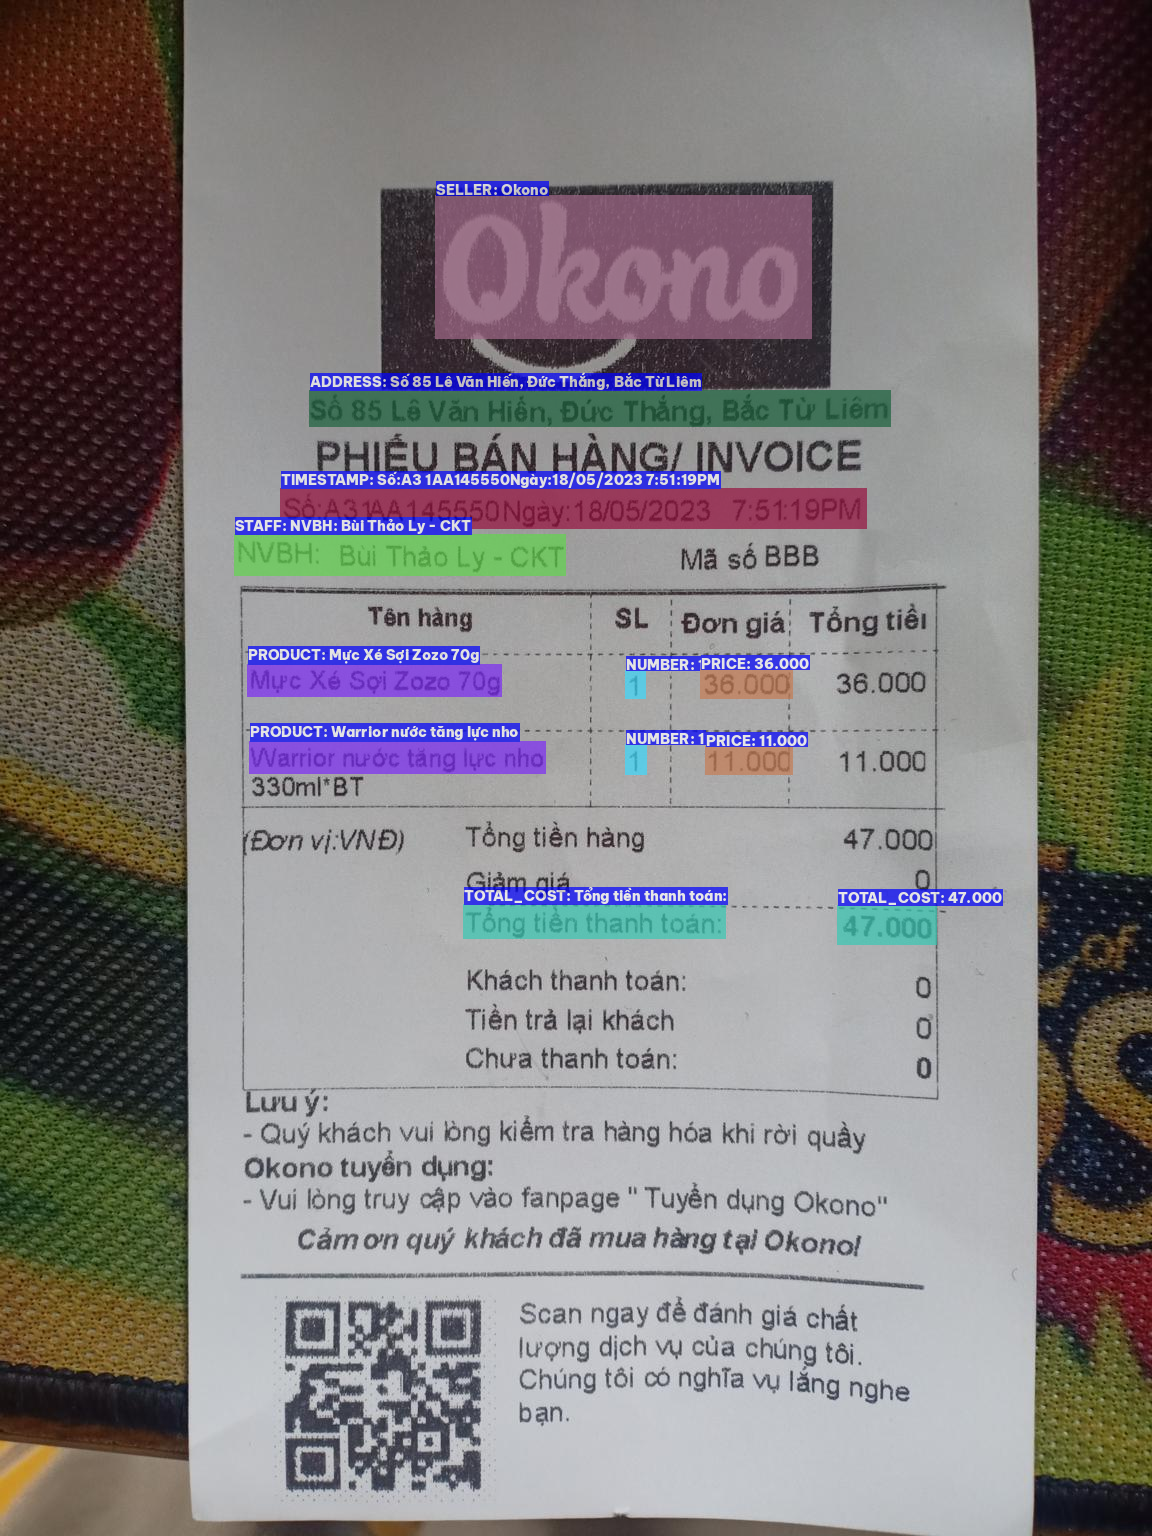
\includegraphics[scale=0.2]{images/dem-image.png}
    \centering
    \caption{Kết quả hình ảnh hóa đơn 1}
\end{figure}

\begin{lstlisting}[language=Python]
{
    "SELLER": "Okono",
    "ADDRESS": "Số 85 Lê Văn Hiến, Đức Thắng, Bắc Từ Liêm",
    "STAFF": "NVBH: Bùi Thảo Ly - CKT",
    "TIMESTAMP": "18/05/2023 7:51:19PM",
    "CODE": "Số:A3 1AA145550",
    "PRODUCTS": [
        {
        "PRODUCT": "Mực Xé Sợi Zozo 70g",
        "NUMBER": "1",
        "PRICE": "36.000"
        },
        {
        "PRODUCT": "Warrior nước tăng lực nho",
        "NUMBER": "1",
        "PRICE": "11.000"
        }
    ],
    "TOTAL_COST": "47.000"
}
\end{lstlisting}

\begin{figure}[h]
    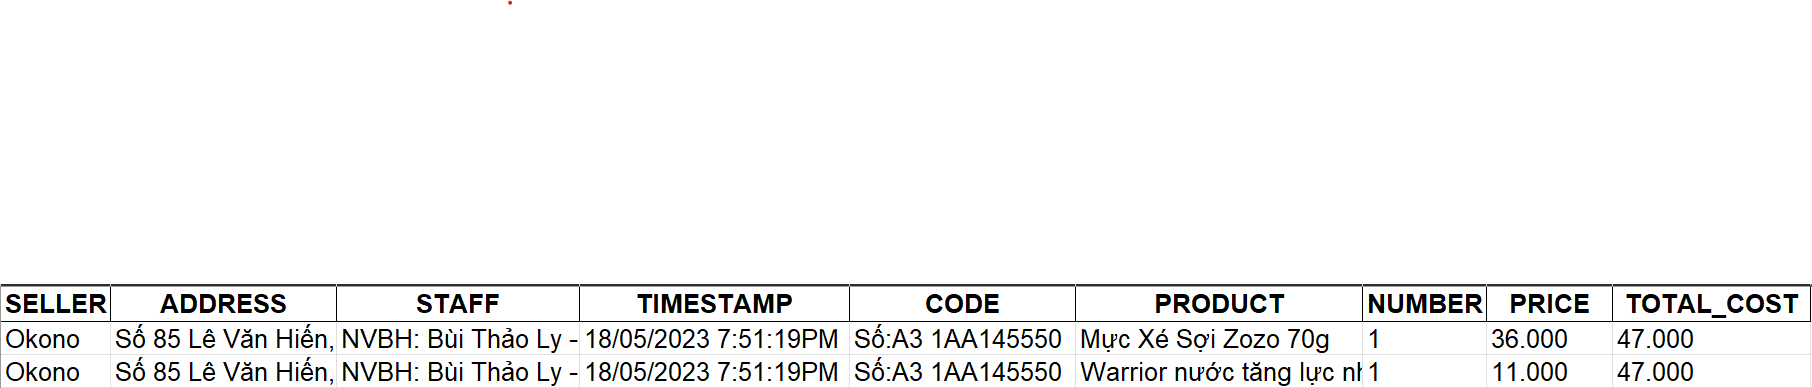
\includegraphics[scale=0.312]{images/result-demi-1.png}
    \caption{Kết quả Excel của hóa đơn 1}
\end{figure}

\paragraph*{Kết quả 2}
\begin{figure}[h]
    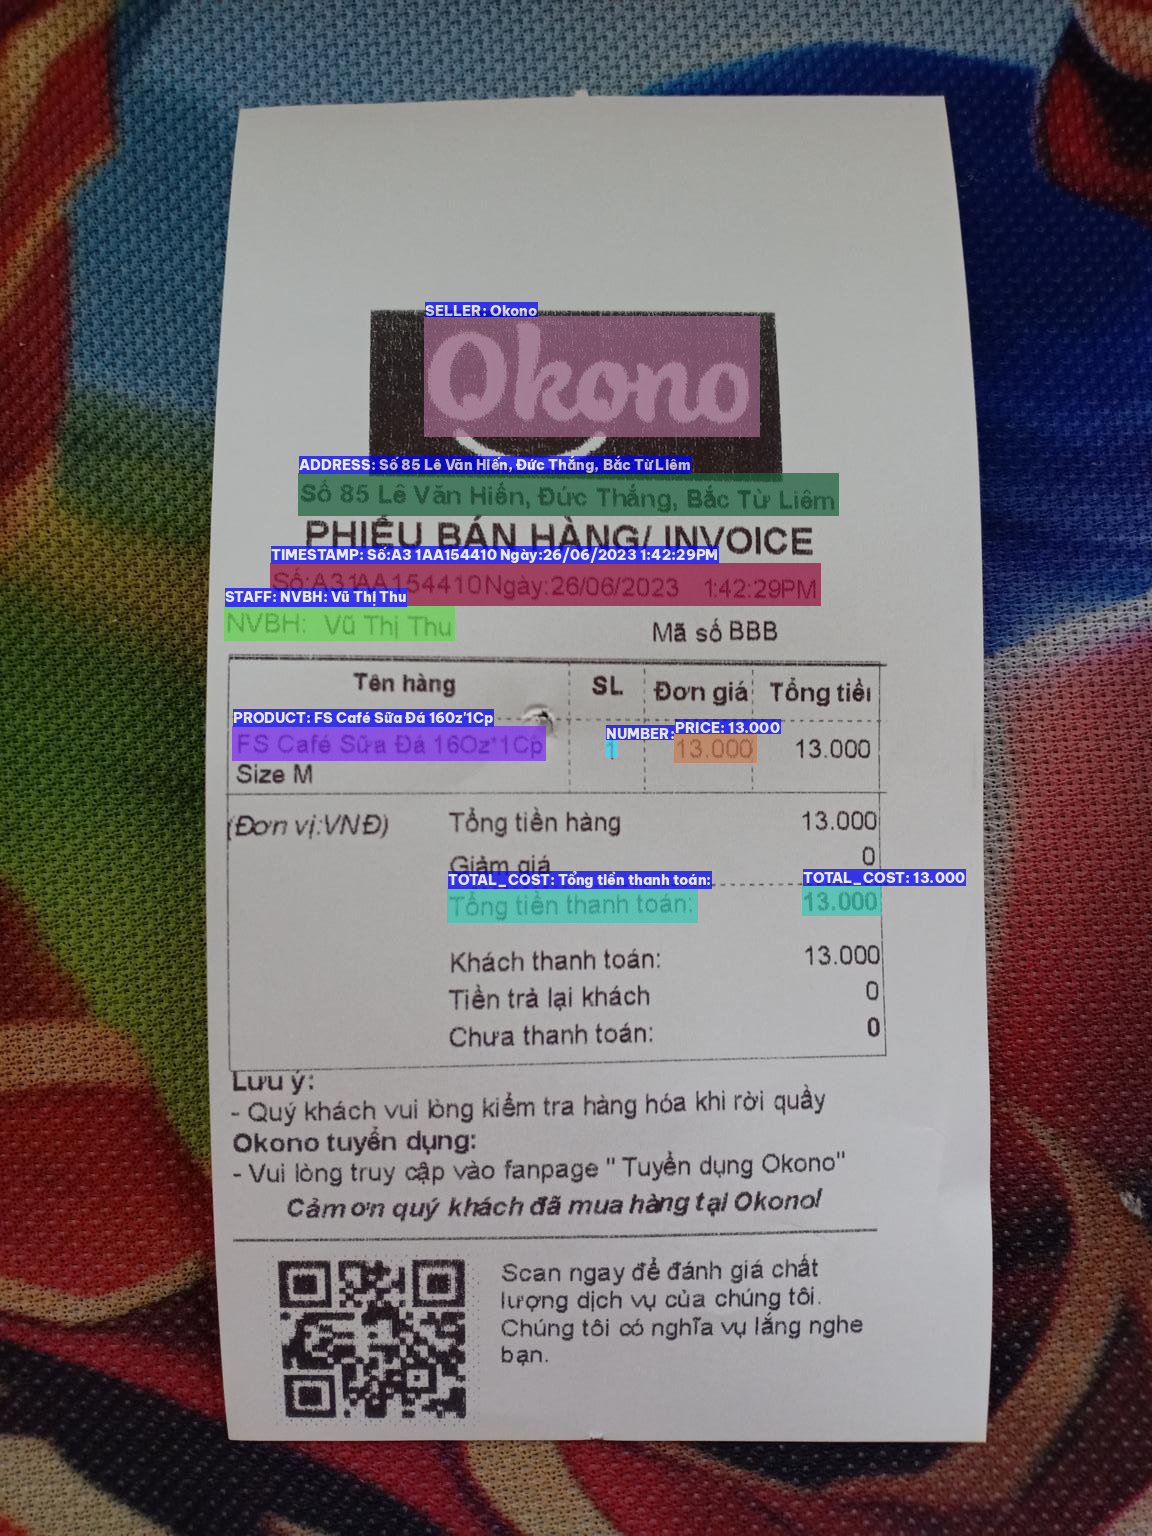
\includegraphics[scale=0.2]{images/demo-image-1.png}
    \centering
    \caption{Kết quả hình ảnh hóa đơn 2}
\end{figure}

\begin{lstlisting}[language=Python]
{
    "SELLER": "Okono",
    "ADDRESS": "Số 85 Lê Văn Hiến, Đức Thắng, Bắc Từ Liêm",
    "STAFF": "NVBH: Vũ Thị Thu",
    "TIMESTAMP": "26/06/2023 1:42:29PM",
    "CODE": "Số:A3 1AA154410",
    "PRODUCTS": [
        {
        "PRODUCT": "FS Café Sữa Đá 160z'1Cp",
        "NUMBER": "1",
        "PRICE": "13.000"
        }
    ],
    "TOTAL_COST": "13.000"
}
\end{lstlisting}

\begin{figure}[h]
    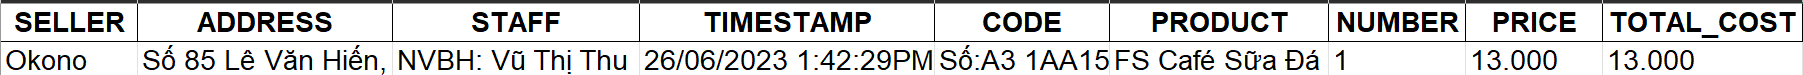
\includegraphics[scale=0.314]{images/result-demo-excel-2.png}
    \caption{Kết quả Excel của hóa đơn 2}
\end{figure}

\paragraph*{Kết quả 3}
\begin{figure}[h]
    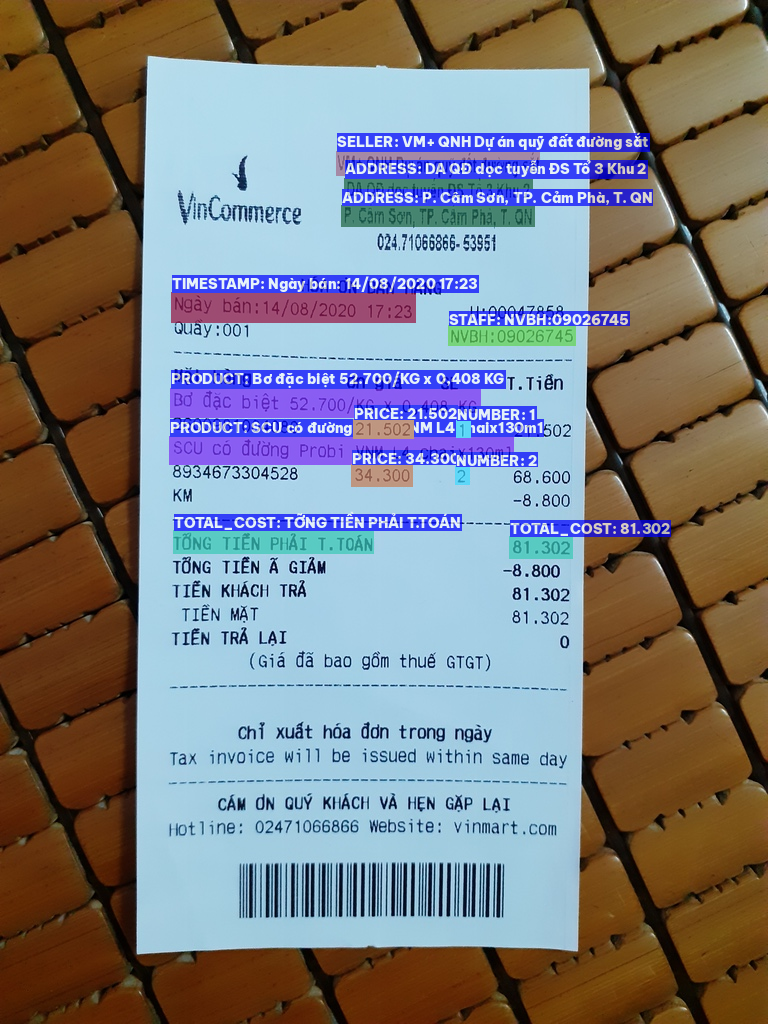
\includegraphics[scale=0.3]{images/demo-image-3.png}
    \centering
    \caption{Kết quả hình ảnh hóa đơn 3}
\end{figure}

\begin{lstlisting}[language=Python]
{
    "SELLER": "VM+ QNH Dự án quỹ đất đường sắt",
    "ADDRESS": "P. Câm Sơn, TP. Cảm Phà, T. QN",
    "STAFF": "NVBH:09026745",
    "TIMESTAMP": "14/08/2020 17:23",
    "CODE": "",
    "PRODUCTS": [
        {
        "PRODUCT": "Bơ đặc biệt 52.700/KG x 0,408 KG",
        "NUMBER": 0,
        "PRICE": 0
        },
        {
        "PRODUCT": "SCU có đường Probi VNM L4 chaix130m1",
        "NUMBER": "2",
        "PRICE": "34.300"
        }
    ],
    "TOTAL_COST": "81.302"
    }
}
\end{lstlisting}

\begin{figure}[h]
    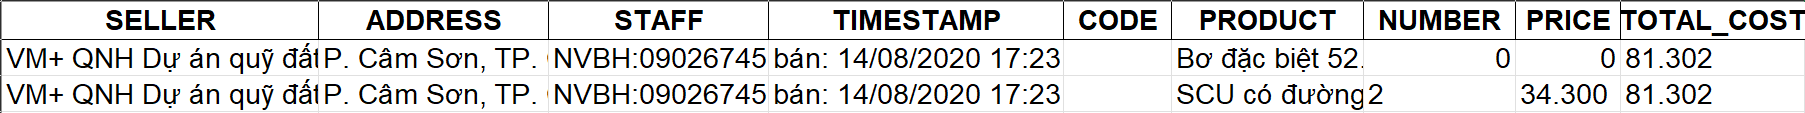
\includegraphics[scale=0.314]{images/result-demo-excel-3.png}
    \caption{Kết quả Excel của hóa đơn 3}
\end{figure}

